\documentclass[12pt,a4paper]{article}

\usepackage[utf8]{inputenc}
\usepackage[T2A]{fontenc}
\usepackage[ukrainian]{babel}
\usepackage{geometry}
\geometry{
    left=2cm,
    right=2cm,
    top=2cm,
    bottom=2cm
}

\usepackage[table]{xcolor}
\usepackage{amsmath}
\usepackage{graphicx}
\usepackage{subcaption}
\usepackage{multirow}
\usepackage{makecell}
\usepackage{pdflscape}
\usepackage{array}
\newcolumntype{C}[1]{>{\centering\arraybackslash}m{#1}}

\usepackage{minted}

\usemintedstyle{vs}
\setminted{linenos, breaklines, frame=single, fontsize=\small}

\RecustomVerbatimCommand{\VerbatimInput}{VerbatimInput}{
    breaklines=true,
    breaksymbolleft={}
}

\usepackage[
  unicode,
  pdftitle={ІО-41, Давидчук А.М., Цифрова схемотехніка, Лабораторна робота №3},
  pdfauthor={Давидчук Артем},
  pdfsubject={Цифрова схемотехніка}
]{hyperref}

\begin{document}

    \begin{titlepage}

        \begin{center}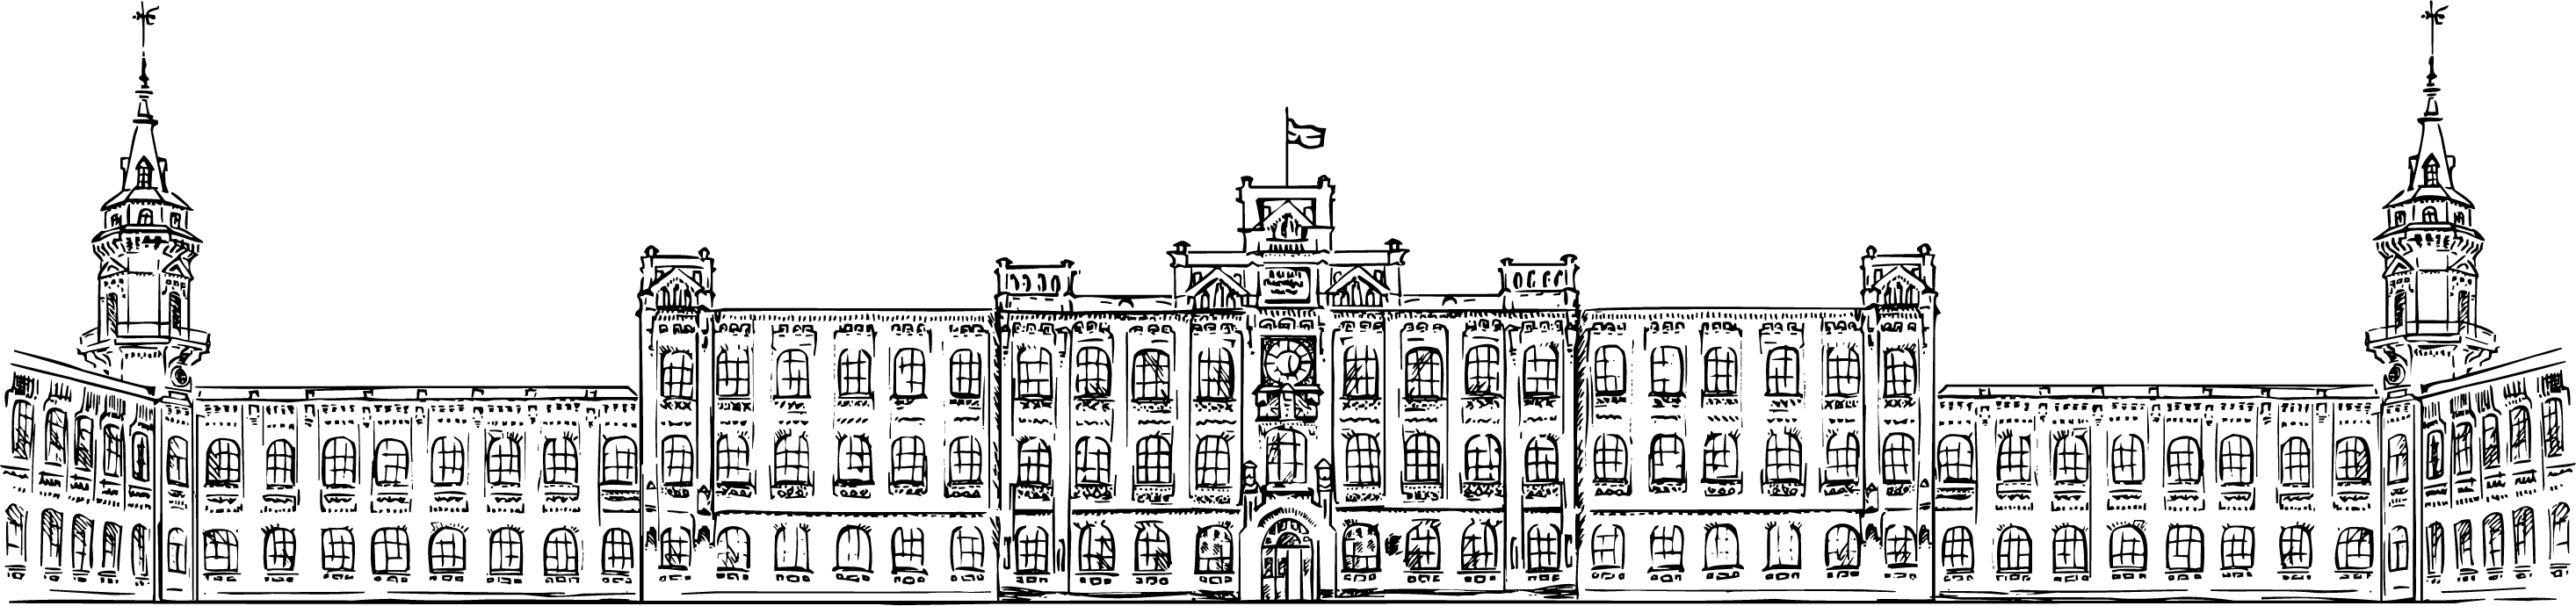
\includegraphics[width=0.7\textwidth]{../../../TITLES/letterhead.png}\end{center}

        \begin{center}
            \large Національний технічний університет України\\
            «Київський політехнічний інститут імені Ігоря Сікорського»\\[1em]
            Факультет інформатики та обчислювальної техніки\\
            Кафедра обчислювальної техніки
        \end{center}

        \vfill

        \begin{center}
            \textbf{\LARGE Цифрова схемотехніка}\\[2em]
            \textbf{\Large Лабораторна робота №3}\\[0.5em]
            «Знайомство з середовищем моделювання ModelSim»
        \end{center}

        \vfill

        \begin{flushright}
            Виконав: студент 2 курсу ФІОТ, гр. ІО-41\\
            \textit{Давидчук А. М.}\\
            Залікова книжка № 4106\\[1em]
            Перевірив: \textit{Нікольський С.\,С.}
        \end{flushright}

        \vfill

        \begin{center}Київ --- 2026\end{center}

    \end{titlepage}

    \noindent
    \textbf{\underline{Тема:}} «Знайомство з середовищем моделювання ModelSim».

    \vspace{1em}

    \begin{center} \textbf{\Large Хід роботи} \end{center}

    \noindent
    Код напівсуматора мовою Verilog:

    \begin{minted}{verilog}
// half_add.v
`timescale 1 ns/1 ps
//------------------------------------------------------
module half_add (S, C, A, B);
    output S, C;
    input A, B;
    wire S, C;
    assign C = A & B;
    assign S = A ^ B;
endmodule
    \end{minted}

    \noindent
    А також файл тестових стимулів (Stim.do):

    \begin{minted}{verilog}
force A 0 0ps, 0 20ps, 1 40ps, 1 60ps;
force B 0 0ps, 1 20ps, 0 40ps, 1 60ps;
    \end{minted}

    Тут вказую часові проміжки саме в пікосекундах, бо резолюція для мого проекту (тривалість кроку) дорівнює 1 пікосекунда.
    Компілюю проект, підключаю Stim.do, та виконую симуляцію (змінюю вхідні аргументи, та фіксую значення виходів напівсуматора). Отримую таку часову діаграму:

    \begin{figure}[h]
        \centering
        
\includegraphics[width=0.8\textwidth]{media/image2.png}
        \caption{Загальне фото проекту}
    \end{figure}

    \newpage

    \begin{figure}[h]
        \centering
        
\includegraphics[width=0.8\textwidth]{media/image1.png}
        \caption{Часова діаграма роботи напівсуматора}
    \end{figure}

    \noindent
    Порівняємо значення виходів в часових діаграмах зі таблицею істинності напівсуматора:

    \begin{table}[h]
        \centering
        \begin{tabular}{|cc|cc|}
        \hline
        $A$ & $B$ & $S$ & $C$ \\
        \hline
        0 & 0 & 0 & 0 \\
        0 & 1 & 1 & 0 \\
        1 & 0 & 1 & 0 \\
        1 & 1 & 0 & 1 \\
        \hline
        \end{tabular}
        \caption{Таблиця істинності напівсуматора: $S=A\oplus B$, $C=A\cdot B$}
    \end{table}

    Як бачимо значення співпадають, що свідить про коректність симуляції та функціонування елементів.

    \begin{center} \textbf{\Large Висновок} \end{center}

    У ході лабораторної роботи було виконано ознайомлення з середовищем моделювання ModelSim та відпрацьовано базовий цикл роботи з HDL-проєктом: створення проєкту, додавання та компіляція Verilog-модуля, запуск симуляції, підключення файлу тестових стимулів (Stim.do) і аналіз часових діаграм. Було реалізовано напівсуматор на мові Verilog, де вихід переносу визначається як $C=A\cdot B$, а вихід суми як $S=A\oplus B$. За результатами моделювання отримані часові діаграми, що повністю відповідають таблиці істинності напівсуматора для всіх комбінацій вхідних сигналів $A$ та $B$. Таким чином, підтверджено коректність реалізованої логічної схеми та засвоєно практичні навички налаштування й проведення моделювання в ModelSim.

\end{document}